

\chapter{Fononi}
\section{Cristallo Armonico "Classico"}
Consideriamo un reticolo di Bravais in cui ogni sito occupato da uno ione non è fisso, ma vibra attorno alla propria posizione di equilibrio. Indichiamo la posizione reale dell'ione con
\[
\vec{r}(\vec{R}) = \vec{R} + \vec{u}(\vec{R}),
\]
dove \(\vec{R}\) è la posizione di equilibrio (proveniente dal reticolo di Bravais) e \(\vec{u}(\vec{R})\) è lo spostamento (con \(|\vec{u}(\vec{R})| \ll a\), dove \(a\) è la distanza interatomica).\\\\
Si assume inoltre l'\textbf{approssimazione adiabatica}, vale a dire che la scala temporale degli elettroni è molto più veloce di quella degli ioni. In questo modo, gli elettroni occupano sempre lo stato fondamentale per una data configurazione ionica, permettendo di disaccoppiare le dinamiche elettronica e ionica.\\\\
L'Hamiltoniana del sistema è data da
\[
H = \sum_{\vec{R}} \frac{\vec{P}(\vec{R})^2}{2M} + U,
\]

\subsection*{Energia Potenziale del Reticolo}
Nel caso statico, cioè quando le ioni restano fissi nelle posizioni di equilibrio, l'energia potenziale si ottiene considerando un potenziale a due corpi:
\[
U = \frac{1}{2}\sum_{\vec{R},\vec{R}'} \phi(\vec{R}-\vec{R}') = \frac{N}{2}\sum_{\vec{R}} \phi(\vec{R}),
\]
dove \(N\) è il numero totale di ioni.\\
Nel caso dinamico, dove gli ioni sono spostati dalle loro posizioni di equilibrio, abbiamo:
\[
U = \frac{1}{2}\sum_{\vec{R},\vec{R}'} \phi\Bigl(\vec{r}(\vec{R}) - \vec{r}(\vec{R}')\Bigr)
= \frac{1}{2}\sum_{\vec{R},\vec{R}'} \phi\Bigl(\vec{R} - \vec{R}' + \vec{u}(\vec{R}) - \vec{u}(\vec{R}')\Bigr).
\]
Poiché \(|\vec{u}(\vec{R})| \ll |\vec{R}|\), è possibile espandere il potenziale in serie di Taylor attorno a \(\vec{u}=0\). Si ottiene:
\begin{equation}
\begin{split}
    U &\approx \frac{N}{2}\sum_{\vec{R} \neq 0}\phi(\vec{R}) \\
    &\quad + \frac{1}{2}\sum_{\vec{R},\vec{R}'} \Bigl\{ \bigl[\vec{u}(\vec{R}) - \vec{u}(\vec{R}')\bigr] \cdot \vec{\nabla} \phi(\vec{R}-\vec{R}') \Bigr\} \\
    &\quad + \frac{1}{4}\sum_{\vec{R},\vec{R}'} \Bigl\{ \bigl[\vec{u}(\vec{R}) - \vec{u}(\vec{R}')\bigr] \cdot \nabla^2 \phi(\vec{R}-\vec{R}') \cdot \bigl[\vec{u}(\vec{R}) - \vec{u}(\vec{R}')\bigr] \Bigr\} \\
    &= U_{\text{eq}} + U_{\text{arm}}.
\end{split}
\end{equation}
Il primo termine \(U_{\text{eq}}\) rappresenta l'energia di equilibrio del reticolo. Il termine lineare è nullo, poiché in un cristallo stabile ci troviamo al minimo dell'energia. Il termine di ordine quadratico \(U_{\text{arm}}\), che descrive la correzione armonica, può essere scritto in due modi equivalenti:
\begin{equation}
    U_{\text{arm}} = \frac{1}{4}\sum_{\vec{R},\vec{R}',\mu,\nu} \bigl[u_{\mu}(\vec{R}) - u_{\mu}(\vec{R}')\bigr]\, \phi_{\mu\nu}\bigl(\vec{R}-\vec{R}'\bigr)\, \bigl[u_{\nu}(\vec{R}) - u_{\nu}(\vec{R}')\bigr],
\end{equation}
oppure
\begin{equation}
    U_{\text{arm}} = \frac{1}{2}\sum_{\vec{R},\vec{R}',\mu,\nu} u_{\mu}(\vec{R})\, D_{\mu\nu}\bigl(\vec{R}-\vec{R}'\bigr)\, u_{\nu}(\vec{R}'),
\end{equation}
dove la \emph{dynamical matrix} (o tensore) è definita da
\[
D_{\mu\nu}\bigl(\vec{R}-\vec{R}'\bigr) = \delta_{\vec{R},\vec{R}'} \sum_{\vec{R}''} \left[\phi_{\mu\nu}\bigl(\vec{R}-\vec{R}'') - \phi_{\mu\nu}\bigl(\vec{R}-\vec{R}'\bigr)\right],
\]
e
\[
\phi_{\mu\nu}(\vec{r}) = \frac{\partial^2 \phi(\vec{r})}{\partial r_\mu \partial r_\nu}.
\]

\subsubsection*{Simmetrie del Sistema}
Il sistema possiede diverse simmetrie:
\begin{enumerate}
    \item L'ordine delle derivate non influenza il risultato, ossia 
    \[(D_{\mu\nu}(\vec{R}-\vec{R}') = D_{\nu\mu}(\vec{R}-\vec{R}')\]
    \item Il tensore \(D\) è simmetrico rispetto allo scambio dei vettori,
     \[(D_{\mu\nu}(\vec{R}-\vec{R}') = D_{\mu\nu}(\vec{R}'-\vec{R})\] 
    \item Se gli ioni si muovono tutti nello stesso modo, cioè \(u_{\mu}(\vec{R}) = d_{\mu}\) per ogni \(\vec{R}\), allora
    \[
    \sum_{\vec{R},\vec{R}'} D_{\mu\nu}(\vec{R}-\vec{R}') = 0,
    \]
    garantendo che le traslazioni uniformi non contribuiscano all'energia (l'energia varia solo rispetto alle deformazioni relative).
\end{enumerate}

\subsection{Equazione del Moto}
L'equazione del moto per gli spostamenti \(\vec{u}(\vec{R})\) si ottiene dalla derivazione rispetto al tempo dell'Hamiltoniana. Si ha:
\begin{equation}
\begin{split}
    M\, \frac{\partial^2 u_{\mu}(\vec{R})}{\partial t^2} &= -\frac{\partial U}{\partial u_{\mu}(\vec{R})} = -\frac{\partial (U_{\text{eq}}+U_{\text{arm}})}{\partial u_{\mu}(\vec{R})} \\
    &= -\sum_{\vec{R}',\nu} D_{\mu\nu}(\vec{R}-\vec{R}')\, u_{\nu}(\vec{R}).
\end{split}
\end{equation}
Il fattore \(1/2\) scompare correttamente durante la derivazione perché, derivando rispetto a \(u_{\mu}(\vec{R})\), si considerano i contributi dovuti sia a \(u_{\mu}(\vec{R})\) che a \(u_{\mu}(\vec{R}')\).

\subsection{Soluzione in 3-D}
La soluzione dell'equazione del moto per un sistema periodico assume la forma di un'onda piana:
\[
\vec{u}(\vec{R},t) = \vec{\varepsilon}\, e^{i(\vec{k}\cdot\vec{R}-\omega t)},
\]
dove \(\vec{\varepsilon}\) è il vettore di polarizzazione (che descrive la direzione delle vibrazioni) e \(\vec{k}\) è il vettore d'onda vibrazionale. Per imporre le condizioni periodiche al contorno (le condizioni di Born--von Karman) si richiede che
\[
\vec{u}(\vec{R}+N_i\vec{a}_i,t) = \vec{u}(\vec{R},t),
\]
da cui il vettore d'onda \(\vec{k}\) deve appartenere al reticolo reciproco e si può scrivere come
\[
\vec{k} = \frac{n_1}{N_1}\vec{b}_1 + \frac{n_2}{N_2}\vec{b}_2 + \frac{n_3}{N_3}\vec{b}_3,
\]
con \(n_i\) interi.

\section{Caso 1-D: Uno Ione per Cella}
Consideriamo ora il caso di una catena unidimensionale di ioni, ad intervallo costante \(a\). Supponiamo che ogni ione sia connesso al suo vicino tramite una "molla" di costante elastica \(K\). La coordinata dell'ione in posizione \(na\) è \(u(na)\).\\
Per la catena unidimensionale, l'energia armonica è data da
\begin{equation}
\begin{split}
    U_{\text{arm}} &= \frac{1}{4}\sum_{n} \Bigl[ u(na) - u\bigl((n+1)a\bigr) \Bigr]^2\, \phi''(a) \\
    &= \frac{1}{2}\sum_{n} \Bigl[ u(na) - u\bigl((n+1)a\bigr) \Bigr]^2\, K,
\end{split}
\end{equation}
dove \(K\) è considerata costante.
Per ricavare l'equazione del moto, deriviamo \(U_{\text{arm}}\) rispetto a \(u(na)\). Tenendo conto dei contributi degli ioni adiacenti, si ottiene:
\begin{equation}
\begin{split}
    M\,\frac{d^2 u(na)}{dt^2} &= -\frac{\partial U_{\text{arm}}}{\partial u(na)} \\
    &=\frac{K}{2}\cdot \bigl[2\cdot\biggr(u(na)-u[(n+1)a]\biggr)\cdot(1)+2\cdot\biggr(u[(n-1)a]-u(na)\biggr)\cdot(-1)\bigr]\\
    &= -K\Bigl[2\,u(na) - u\bigl((n+1)a\bigr) - u\bigl((n-1)a\bigr)\Bigr].
\end{split}
\end{equation}
Per risolvere quest'equazione, assumiamo una soluzione del tipo onda piana:
\[
u(na,t) = \varepsilon\, e^{i( kna - \omega t)},
\]
con \(k\) assunto quantizzato dalle condizioni di Born--von Karman, \(e^{ikNa} = 1\) (da cui \(k = \frac{2\pi}{Na}n\), con \(n\) intero). Sostituendo questa soluzione nell'equazione del moto si ha:
\[
-M\omega^2\, e^{i( kna-\omega t)} = -K\, e^{i( kna-\omega t)} \left[2 - e^{ika} - e^{-ika}\right].
\]
Dividendo per il termine esponenziale, e utilizzando la relazione
\[
2 - e^{ika} - e^{-ika} = 2\Bigl[1-\cos(ka)\Bigr] = 4\sin^2\Bigl(\frac{ka}{2}\Bigr),
\]
si ottiene:
\[
M\omega^2 = 4K\,\sin^2\left(\frac{ka}{2}\right),
\]
quindi la dispersione è data da:
\[
\omega(k) = 2\sqrt{\frac{K}{M}}\, \Bigl|\sin\Bigl(\frac{ka}{2}\Bigr)\Bigr|.
\]
Nel limite in cui \(k\to 0\), espandendo la funzione \(\sin(ka/2)\) per piccoli \(ka\) si ha:
\[
\omega(k) \approx 2\sqrt{\frac{K}{M}}\,\frac{ka}{2} = \sqrt{\frac{K}{M}}\, a\, k,
\]
ossia la relazione diventa lineare, e le velocità di fase e di gruppo coincidono:
\[
v_f = \frac{\omega}{k} = v_g = \sqrt{\frac{K}{M}}\, a.
\]

\section{Caso 1-D: Soluzione con la Dynamical Matrix}
Consideriamo il caso generico in 3-D e poi specializziamo al caso unidimensionale. L'equazione del moto è:
\begin{equation}
    M\,\frac{\partial^2 u_{\mu}(\vec{R})}{\partial t^2} = -\sum_{\vec{R}',\nu} D_{\mu\nu}(\vec{R}-\vec{R}')\, u_{\nu}(\vec{R}).
\end{equation}
Cerchiamo soluzioni del tipo:
\[
u_{\mu}(\vec{R},t) = \varepsilon_{\mu}\, e^{i(\vec{k}\cdot\vec{R} - \omega t)}.
\]
Scegliendo l'origine, ad esempio \(\vec{R}=0\), l'equazione diventa:
\begin{equation}
    -M\,\omega^2\, \vec{\varepsilon}\, e^{i(\vec{k}\cdot\vec{0} - \omega t)} = -\sum_{\vec{R}'} D(\vec{R}')\, \vec{\varepsilon}\, e^{i(\vec{k}\cdot\vec{R}' - \omega t)}.
\end{equation}
Quindi,
\[
M\,\omega^2\, \vec{\varepsilon} = \sum_{\vec{R}'} D(\vec{R}')\, \vec{\varepsilon}\, e^{i\vec{k}\cdot\vec{R}'}.
\]
Definiamo la trasformata discreta della dynamical matrix nel \(\vec{k}\)-spazio:
\[
D(\vec{k}) = \sum_{\vec{R}'} D(\vec{R}')\, e^{i\vec{k}\cdot\vec{R}'}.
\]
Utilizzando le proprietà simmetriche e dividendo la somma in due parti (una con \(\vec{R}'\) e una con \(-\vec{R}'\)), otteniamo:
\begin{equation}
\begin{split}
    D(\vec{k}) &= \frac{1}{2}\sum_{\vec{R}'} D(\vec{R}') \Bigl[e^{i\vec{k}\cdot\vec{R}'} + e^{-i\vec{k}\cdot\vec{R}'}\Bigr] \\
    &= \sum_{\vec{R}'} D(\vec{R}') \Bigl[\cos(\vec{k}\cdot\vec{R}') - 1\Bigr] \quad \text{(poiché la somma costante \(\sum_{\vec{R}'} D(\vec{R}') = 0\))} \\
    &= -2 \sum_{\vec{R}'} D(\vec{R}') \, \sin^2\Bigl(\frac{\vec{k}\cdot\vec{R}'}{2}\Bigr).
\end{split}
\end{equation}
Specializzando al caso unidimensionale, dove gli unici contributi significativi sono dovuti ai vicini immediati (cioè, \(n = \pm 1\)):
\[
M\,\omega^2 = -2 \sum_{n} D(na)\, \sin^2\left(\frac{k\,na}{2}\right).
\]
Per il caso unidimensionale, se consideriamo che il contributo di \(D(na)\) è:
\[
D(na) = \begin{cases}
-K, & \text{per } n = \pm 1, \\
D(0) = 2K, & \text{per } n = 0,
\end{cases}
\]
e notiamo che \(\sin(0)= 0\), l'unico contributo viene dai primi vicini:
\[
M\,\omega^2 = -2\Bigl[D(a)\,\sin^2\Bigl(\frac{ka}{2}\Bigr) + D(-a)\,\sin^2\Bigl(\frac{-ka}{2}\Bigr)\Bigr].
\]
Dati \(D(a)=D(-a)=-K\) e ricordando che \(\sin^2\bigl(\frac{-ka}{2}\bigr)=\sin^2\bigl(\frac{ka}{2}\bigr)\), otteniamo:
\[
M\,\omega^2 = -2\Bigl[ -K\,\sin^2\Bigl(\frac{ka}{2}\Bigr) -K\,\sin^2\Bigl(\frac{ka}{2}\Bigr) \Bigr] = 4K\,\sin^2\Bigl(\frac{ka}{2}\Bigr).
\]
Pertanto,
\[
\omega^2(k) = \frac{4K}{M}\, \sin^2\left(\frac{ka}{2}\right)
\quad \Longrightarrow \quad
\omega(k) = 2\sqrt{\frac{K}{M}}\, \left|\sin\left(\frac{ka}{2}\right)\right|.
\]
Questa espressione rappresenta la relazione di dispersione per i fononi in una catena unidimensionale di ioni, ottenuta sia tramite il metodo diretto che utilizzando la dinamical matrix.
\bigskip
Per \(k \to 0\) espandendo la funzione \(\sin(x)\) per piccoli \(x\) si ha:
\[
\sin\left(\frac{ka}{2}\right) \approx \frac{ka}{2},
\]
da cui:
\[
\omega(k) \approx \sqrt{\frac{K}{M}}\, a\, k.
\]
In questo limite lineare, le velocità di fase e di gruppo coincidono:
\[
v_f = \frac{\omega}{k} \approx \sqrt{\frac{K}{M}}\, a
\quad \text{e} \quad
v_g = \frac{d\omega}{dk} \approx \sqrt{\frac{K}{M}}\, a.
\]


\section{Caso 1-D, Due Ioni per Cella}
Consideriamo ora il caso in cui la cella unitaria contiene due ioni. 
\begin{figure} [H]
    \centering
    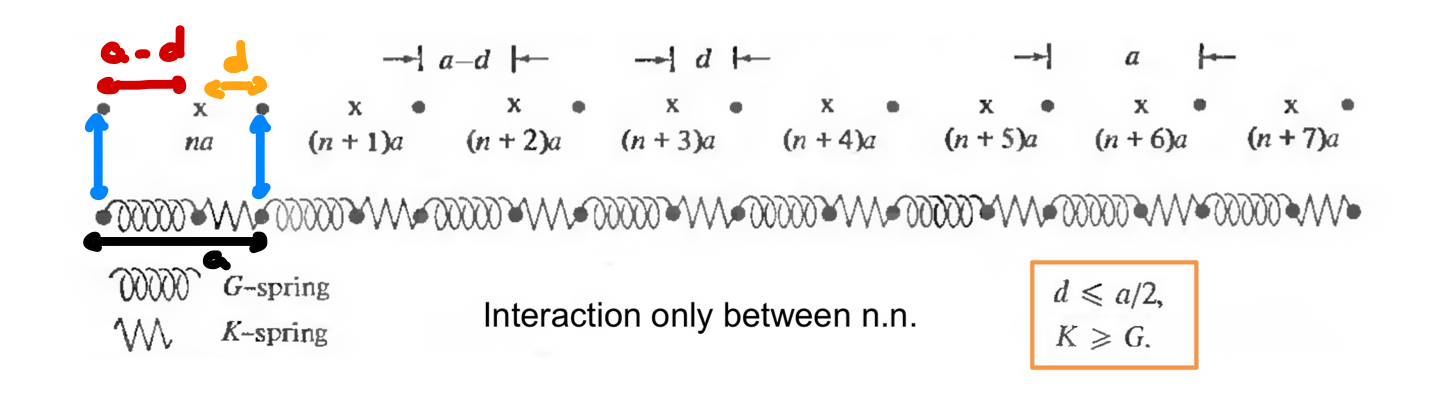
\includegraphics[width=1\textwidth]{images/8-Fononi/Fononi.jpeg}
    \caption{}
\end{figure}

\begin{itemize}
    \item Supponiamo che vi siano due costanti elastiche differenti, denotate da \(G\) e \(K\), e due posizioni di equilibrio differenti: un ione oscilla attorno a \(na\) e l'altro attorno a \(na+d\), con \(d\leq \frac{a}{2}\)
    \item In questo sistema le forze che agiscono tra gli ioni dipendono dalla loro separazione: gli ioni separati da \(d\) interagiscono con una costante elastica \(K\), mentre quelli separati da \(a-d\) interagiscono con una costante \(G\). 
    \item \(K \geq G\), ossia il legame interno (tra ioni in posizione \(na\) e \(na+d\)) è più forte, il che rompe la simmetria del sistema e porta all'esistenza di due branche (acustica e ottica).
\end{itemize}
Definiamo $u_1(na)$ per lo ione che oscilla attorno a $na$, $u_2(na)$ per lo ione che oscilla attorno a $na+d$.\\
L'energia armonica totale del sistema si scrive come:
\begin{equation}
\begin{split}
    U_{\text{arm}} &= \frac{K}{2}\sum_{n} \Bigl[u_1(na) - u_2(na)\Bigr]^2 
    + \frac{G}{2}\sum_{n} \Bigl[u_2(na) - u_1\bigl((n+1)a\bigr)\Bigr]^2.
\end{split}
\end{equation}
Le equazioni del moto per i due ioni si ottengono derivando \(U_{\text{arm}}\) rispetto a \(u_1(na)\) e \(u_2(na)\):
\begin{enumerate}
    \item Per \(u_1(na)\):
    \begin{equation}
    M\,\frac{\partial^2 u_1(na)}{\partial t^2} = -\frac{\partial U}{\partial u_1(na)} = -K\Bigl[u_1(na) - u_2(na)\Bigr] - G\Bigl[u_1(na) - u_2\bigl((n-1)a\bigr)\Bigr].
    \end{equation}
    \item Per \(u_2(na)\):
    \begin{equation}
    M\,\frac{\partial^2 u_2(na)}{\partial t^2} = -\frac{\partial U}{\partial u_2(na)} = -K\Bigl[u_2(na) - u_1(na)\Bigr] - G\Bigl[u_2(na) - u_1\bigl((n+1)a\bigr)\Bigr].
    \end{equation}
\end{enumerate}
Si cerca la soluzione in forma d'onda, ponendo:
\[
u_1(na,t) = \varepsilon_1\, e^{i( kna - \omega t)},\quad
u_2(na,t) = \varepsilon_2\, e^{i( kna - \omega t)}.
\]
Sostituendo queste soluzioni nelle equazioni del moto e dividendo per \(e^{i( kna - \omega t)}\) si ottengono due equazioni algebriche:
\begin{align}
    -M\omega^2\,\varepsilon_1 &= -K\Bigl[\varepsilon_1 - \varepsilon_2\Bigr] - G\Bigl[\varepsilon_1 - \varepsilon_2\,e^{-ika}\Bigr],\\[1mm]
    -M\omega^2\,\varepsilon_2 &= -K\Bigl[\varepsilon_2 - \varepsilon_1\Bigr] - G\Bigl[\varepsilon_2 - \varepsilon_1\,e^{ika}\Bigr].
\end{align}
Riarrangiando:
\begin{align}
    \Bigl[M\omega^2 - (K+G)\Bigr]\varepsilon_1 + \Bigl[K + G\,e^{-ika}\Bigr]\varepsilon_2 &= 0, \\
    \Bigl[K + G\,e^{ika}\Bigr]\varepsilon_1 + \Bigl[M\omega^2 - (K+G)\Bigr]\varepsilon_2 &= 0.
\end{align}
Per avere una soluzione non banale il determinante del sistema deve essere nullo:
\begin{equation}
\begin{split}
    \Bigl[M\omega^2 - (K+G)\Bigr]^2 &- \Bigl[K + G\,e^{-ika}\Bigr]\Bigl[K + G\,e^{ika}\Bigr] = 0.
\end{split}
\end{equation}
Osserviamo che
\[
\Bigl[K + G\,e^{-ika}\Bigr]\Bigl[K + G\,e^{ika}\Bigr] = K^2 + KG\Bigl(e^{ika}+e^{-ika}\Bigr) + G^2,
\]
e poiché
\[
e^{ika}+e^{-ika} = 2\cos(ka),
\]
si ottiene:
\[
\Bigl[M\omega^2 - (K+G)\Bigr]^2 - \Bigl[K^2 + 2KG\cos(ka) + G^2\Bigr] = 0.
\]
Pertanto, l'equazione si scrive:
\[
M^2\omega^4 - 2M\omega^2(K+G) + (K+G)^2 - \Bigl[K^2 + 2KG\cos(ka) + G^2\Bigr] = 0.
\]
Notiamo che
\[
(K+G)^2 - \Bigl[K^2 + 2KG\cos(ka) + G^2\Bigr] = 2KG\bigl[1-\cos(ka)\bigr],
\]
per cui l'equazione diventa:
\[
M^2\omega^4 - 2M\omega^2(K+G) + 2KG\bigl[1-\cos(ka)\bigr] = 0.
\]
Da cui:
\[
\omega^2 = \frac{K+G}{M} \pm \frac{1}{M}\sqrt{K^2 + G^2 + 2KG\cos(ka)}.
\]
Le due soluzioni corrispondono alle due branche:
\begin{itemize}
    \item La \textbf{branca ottica}: per cui le oscillazioni dei due ioni sono in controfase.
    \item La \textbf{branca acustica}: in cui le oscillazioni dei due ioni avvengono in fase.
\end{itemize}
In casi limite si ha:
\begin{enumerate}
    \item Per \(k=0\): si ottengono le soluzioni
    \[
    \omega = 0 \quad \text{(branca acustica)}
    \]
    e
    \[
    \omega = \sqrt{2\frac{K+G}{M}} \quad \text{(branca ottica).}
    \]
    \item Al bordo della prima zona di Brillouin (\(k = \pi/a\)), si ottengono due soluzioni:
    \[
    \omega_1^2 = \frac{K+G}{M} + \frac{K-G}{M} = \frac{2K}{M} \quad \text{(branca ottica)}
    \]
    e
    \[
    \omega_2^2 = \frac{K+G}{M} - \frac{K-G}{M} = \frac{2G}{M} \quad \text{(branca acustica).}
    \]
\end{enumerate}
La relazione tra le due branche è schematizzata nella Figura~\ref{fig:branche}. Nella branca ottica, i due atomi oscillano in controfase, generando dipoli che interagiscono fortemente con la luce (particolarmente importante nei cristalli ionici), mentre nella branca acustica i due atomi oscillano in fase.
\begin{figure} [H]
    \centering
    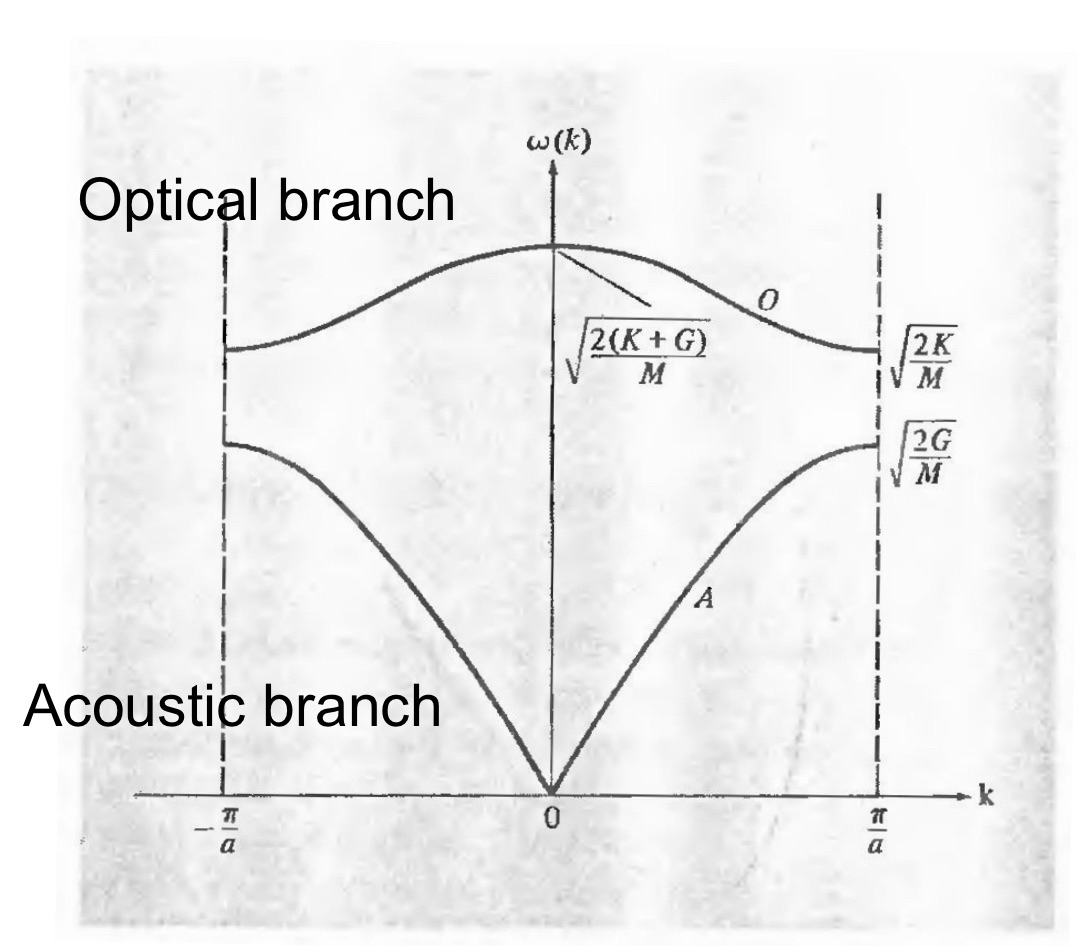
\includegraphics[width=0.7\textwidth]{images/8-Fononi/Branche.jpeg}
    \caption{}
    \label{fig:branche}
\end{figure}

\subsection{Considerazioni Generali}
La trasformata discreta della dynamical matrix, \(\mathbf{D}(\vec{k})\), è un tensore simmetrico e possiede 3 autovettori reali, \(\vec{\varepsilon}_s(\vec{k})\), che corrispondono agli stati normali di vibrazione, dove \(s\) è l'indice di branca. Questi soddisfano:
\begin{equation}
    \mathbf{D}(\vec{k})\,\vec{\varepsilon}_s(\vec{k}) = \lambda_s(\vec{k})\, \vec{\varepsilon}_s(\vec{k}),
\end{equation}
da cui si ricava la relazione di dispersione dei modi normali:
\[
\omega_s(\vec{k}) = \sqrt{\frac{\lambda_s(\vec{k})}{M}}.
\]
Per ogni valore di \(\vec{k}\) in uno spazio tridimensionale, se la cella unitaria contiene \(N\) ioni, ci sono in totale \(3N\) modi normali: in particolare, vi sono 3 branche acustiche (per cui il numero di modi che contribuiscono alla vibrazione traslazionale comune) e \(3(N-1)\) branche ottiche (relative ai movimenti relativi tra gli ioni all'interno della cella).\\
Questi autostati rappresentano, in maniera quantistica, i pacchetti d'onda dei modi normali di vibrazione del solido.



%\section{Misurazione dei fononi}
%Per misurare i fononi c'è bisogno di qualcosa che scatterando con loro ci dia delle informazioni riguardo al loro momento. Utilizzo delle particelle non cariche perché non voglio che ci sia interazione con gli elettroni, dei candidati potrebbero essere quindi i neutroni oppure i fotoni che però sono in un range di energia-momento molto differenti
%\[ \begin{split}
%    &\text{neutroni:} \ \ E_n = \frac{p^2}{2M_n}, \ \ M_n = 1838,65 \ m_e \\
%    &\text{fotoni}: \ \ E_\gamma= pc
%\end{split}\]
%Guardando il grafico in Figura \ref{disp fon} si nota che con i fotoni riesco ad osservare piccoli valori di k quindi sono buoni per controllare la parte centrale della zona di Brillouin poiché è molto vicino a zero, mentre coi neutroni riesco a vedere un'area più grande.
%\begin{figure} [H]
%    \centering
%    
\includegraphics[width=0.5\linewidth]{dispersionefononi.png}
 %   \caption{le linee orizzontali indicano il range energetico dell'energia termica e quindi dei fononi, $E_\gamma$ è l'energia dei fotoni mentre $E_n$ è quella dei neutroni}
 %   \label{disp fon}
%\end{figure} 
%Quindi irraggiando un cristallo con un fascio di neutroni possiamo vedere la perdita (o guadagno) di energia del neutrone che interagisce col cristallo come un fenomeno dovuto all'emissione (o assorbimento) di un fonone e andando a vedere l'angolo di uscita e l'energia dei neutroni uscenti ottengo informazioni sullo spettro fononico. 
%\\~\\
%Considero un neutrone di momento $\mathbf{p}$ ed energia $E = \frac{p^2}{2M_n}$ che in seguito all'urto con un cristallo fuoriesce da esso con momento $\mathbf{p}'$ ed energia $E'=\frac{p'^2}{2M_n}$. \\
%Il neutrone entrando nel solido interagisce con uno o più atomi e causa una vibrazione, quindi in pratica la particella esterna interagisce con un modo normale e scambia un quanto di energia vibrazionale, quel quanto di energia vibrazionale è il fonone. Supponiamo che inizialmente il fonone si trova in uno stato con un numero di occupazione pari a $n_{ks}$ e in seguito all'urto troviamo il cristallo in uno stato nel quale il numero di occupazione dei fononi è $n_{ks}'$, quindi per la conservazione dell'energia abbiamo che:
%\[ \begin{split}
%    &\Delta E = E'-E = -\sum_{ks} \hbar\omega_{ks} \Delta n_{ks} \\
%    & \Delta n_{ks} = n_{ks}'-n_{ks}
%\end{split}\]
%Quindi il cambio dell'energia del neutrone è pari all'energia del fonone che ha assorbito passando attraverso al cristallo meno l'energia del fonone che ha emesso. (s è l'indice della branca). \\
%Invece per quanto riguarda la conservazione del momento, il cambiamento nel momento del neutrone è pari all'inverso del momento cristallino totale del fonone più un vettore del reticolo reciproco
%\[ \Delta p = p' - p = -\sum_{ks} \hbar\mathbf{k} \Delta n_{ks} + \text{vettore reticolo reciproco} \times \hbar\]
%Guardando $\Delta E$ e $\Delta p$ posso ricostruire il grafico in Figura \ref{Branche}. \\
%Ricorda però che il momento cristallino del fonone non è in generale un momento come lo conosciamo. Il "momento cristallino" è semplicemente $\hbar$-volte il vettore d'onda del fonone. Si chiama così perché spesso ha un ruolo simile a quello del momento ma il fatto è che non è soggetto in maniera rigida alla conservazione del momento, la sua simmetria è quella di un reticolo di Bravais e per questo la sua legge di conservazione non è rigida come quella della conservazione del momento ma si conserva sempre più o meno un vettore del reticolo reciproco. \\
%Ora esaminiamo la distribuzione dei nuetroni scatterati emergenti dal cristallo classificando i tipi di scattering che possoo avvenire a seconda del numero totale di fononi con i quali i neutroni scambiano energia passando attraverso al cristallo. 

\section{Misurazione dei Fononi}
Per misurare i fononi all'interno di un cristallo, è necessario utilizzare particelle che possano interagire con essi senza essere significativamente influenzate dagli elettroni. Per questo motivo si prediligono particelle neutre, come i neutroni o i fotoni, che offrono caratteristiche energetiche e di impulso differenti.
\begin{equation}
\begin{split}
&\text{Neutroni:} \quad E_n = \frac{p^2}{2M_n}, \quad M_n = 1838.65\, m_e \\
&\text{Fotoni:} \quad E_\gamma = pc
\end{split}
\end{equation}
Dal confronto tra le relazioni energia-momento si deduce che:
\begin{itemize}
    \item  I fotoni hanno un impulso più piccolo rispetto alla loro energia, rendendoli adatti per esplorare la zona centrale della prima zona di Brillouin, ovvero per bassi valori del vettore d'onda $\mathbf{k}$.
    \item I neutroni, avendo massa e quindi una diversa relazione tra energia e impulso, riescono a coprire una porzione più ampia della zona di Brillouin.
\end{itemize}
\begin{figure}[H]
    \centering
    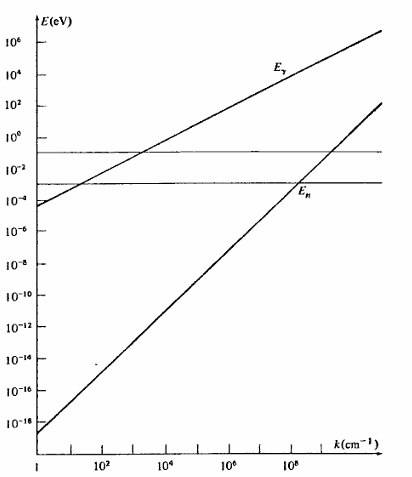
\includegraphics[width=0.5\linewidth]{images/8-Fononi/dispersionefononi.png}
    \caption{Le linee orizzontali rappresentano il range energetico tipico dell'energia termica e quindi dei fononi. $E_\gamma$ rappresenta l'energia dei fotoni, mentre $E_n$ quella dei neutroni.}
    \label{fig:disp-fon}
\end{figure}

L'irraggiamento di un cristallo con un fascio di neutroni permette di analizzare l'interazione tra i neutroni incidenti e i fononi all'interno del reticolo cristallino. Quando un neutrone interagisce con un fonone, può assorbirlo o emetterlo, modificando la propria energia e direzione di moto.\\\\
\textbf{Misurando l'energia e la direzione del neutrone dopo l'interazione, si possono ottenere informazioni sullo spettro fononico del materiale.}\\\\
Consideriamo un neutrone con momento iniziale $\mathbf{p}$ ed energia $E = \frac{p^2}{2M_n}$ che, dopo l'interazione, esce dal cristallo con momento $\mathbf{p}'$ ed energia $E' = \frac{p'^2}{2M_n}$.\\
Durante l'interazione, il neutrone può scambiare energia con i modi vibrazionali del cristallo, ovvero con i fononi. \\
Se inizialmente il fonone si trova in uno stato caratterizzato da un numero di occupazione $n_{\mathbf{k}s}$, al termine dell'interazione tale numero diventa $n_{\mathbf{k}s}'$.\\\\
La variazione di energia del neutrone è quindi data da:
\begin{equation}
\begin{split}
\Delta E &= E' - E = - \sum_{\mathbf{k}s} \hbar \omega_{\mathbf{k}s} (n_{\mathbf{k}s}' - n_{\mathbf{k}s}) \\
         &= - \sum_{\mathbf{k}s} \hbar \omega_{\mathbf{k}s} \Delta n_{\mathbf{k}s}
\end{split}
\end{equation}
Dove $s$ rappresenta l'indice della branca fononica. \textbf{La variazione di energia del neutrone è quindi pari all'energia totale dei fononi emessi meno quella dei fononi assorbiti durante l'interazione.}\\
La conservazione del momento cristallino, invece, implica che:
\begin{equation}
\Delta \mathbf{p} = \mathbf{p}' - \mathbf{p} = - \sum_{\mathbf{k}s} \hbar \mathbf{k} \Delta n_{\mathbf{k}s} + \hbar \mathbf{K}
\end{equation}
Dove $\mathbf{K}$ è un vettore del reticolo reciproco. Questo termine riflette la natura periodica del reticolo cristallino: \textbf{il momento cristallino non si conserva rigidamente come il momento canonico, ma si conserva a meno di $\pm$ un vettore del reticolo reciproco, a causa della simmetria discreta del reticolo di Bravais.\\
Il "momento cristallino" del fonone, definito come $\hbar \mathbf{k}$, non è un vero e proprio momento nel senso classico, ma un'entità legata alla simmetria traslazionale del cristallo.}\\\\
Analizzando la variazione di energia e momento del neutrone in seguito all'interazione, si può ricostruire la relazione di dispersione dei fononi.\\\\

Infine, classificando i neutroni usciti dal cristallo in base alla variazione totale di numero di fononi ($\sum_{\mathbf{k}s} |\Delta n_{\mathbf{k}s}|$), si può distinguere tra:
\begin{itemize}
    \item \textbf{Scattering elastico}: nessun fonone è creato o distrutto ($\Delta n_{\mathbf{k}s} = 0$), l'energia del neutrone resta invariata.
    \item \textbf{Scattering anelastico}: avviene creazione o annichilazione di fononi ($\Delta n_{\mathbf{k}s} \neq 0$), l'energia del neutrone cambia, fornendo informazioni sullo spettro fononico del materiale.
\end{itemize}
Questa tecnica prende il nome di "inelastic neutron scattering" e costituisce uno degli strumenti fondamentali per lo studio delle eccitazioni vibrazionali nei solidi.
\subsection{Zero Phonon Scattering}
In questo caso lo stato finale del cristallo coincide esattamente con quello iniziale, pertanto non viene scambiata energia tra il neutrone e il reticolo. La conservazione del momento cristallino impone che il vettore d'onda del neutrone possa cambiare solo di un multiplo di $\hbar\mathbf{K}$, dove $\mathbf{K}$ è un vettore del reticolo reciproco. Se indichiamo il momento iniziale e finale del neutrone con 
\[
\mathbf{p} = \hbar \mathbf{q} \quad \text{e} \quad \mathbf{p}' = \hbar \mathbf{q}',
\]
i vincoli imposti sono:
\[
\mathbf{q}' = \mathbf{q} \quad \text{oppure} \quad \mathbf{q}' = \mathbf{q} + \mathbf{K}.
\]
Queste condizioni sono le \emph{condizioni di Von Laue} (vedi sezione \ref{subsec:Formulazione-di-Von-Laue}) che, analogamente alla diffrazione di raggi X, determinano i picchi di Bragg. In altre parole, un fascio di neutroni, trattato come un'onda piana con vettore d'onda $\mathbf{q}$, scattera elasticamente solo nelle direzioni che soddisfano queste condizioni. Di conseguenza, tale scattering fornisce informazioni precise sulla struttura cristallina senza coinvolgere processi di eccitazione vibrazionale.

\subsection{One-Phonon Scattering}
Nel caso in cui il neutrone assorbe o emette un singolo fonone, la maggior parte delle informazioni sullo spettro vibrazionale viene trasferita in un unico evento. La conservazione di energia e di momento (tenendo conto del vettore di compensazione del reticolo $\hbar\mathbf{K}$) viene espressa nei seguenti due casi:

\paragraph{Assorbimento di un Fonone}
Il neutrone assorbe un fonone caratterizzato dal vettore d'onda $\mathbf{k}$ e dalla frequenza $\omega_s(\mathbf{k})$, dove $s$ indica la branca fononica. Le relazioni di conservazione sono:
\[
\begin{split}
E' &= E + \hbar \omega_s(\mathbf{k}), \\
\mathbf{p}' &= \mathbf{p} + \hbar \mathbf{k} + \hbar \mathbf{K} = \mathbf{p} + \hbar \left( \mathbf{k} + \mathbf{K} \right).
\end{split}
\]

\paragraph{Emissione di un Fonone}
In questo caso il neutrone emette un fonone e quindi perde un quanto di energia pari a $\hbar \omega_s(\mathbf{k})$. Le condizioni di conservazione diventano:
\[
\begin{split}
E' &= E - \hbar \omega_s(\mathbf{k}), \\
\mathbf{p}' &= \mathbf{p} - \hbar \mathbf{k} + \hbar \mathbf{K} = \mathbf{p} + \hbar \left( \mathbf{K} - \mathbf{k} \right).
\end{split}
\]

Si noti che, dal momento che $\omega_s(\mathbf{k})$ è una funzione periodica nel reticolo reciproco (cioè $\omega_s(\mathbf{k}) = \omega_s(\mathbf{k} \pm \mathbf{K})$), possiamo definire il vettore d'onda del fonone in funzione della variazione di momento del neutrone. Infatti, ignorando esplicitamente il contributo del vettore reticolo $\mathbf{K}$, si ottengono le seguenti relazioni:
\[
\begin{split}
\mathbf{k} &= \frac{\mathbf{p}' - \mathbf{p}}{\hbar} \quad \text{(fonone assorbito)}, \\
\mathbf{k} &= \frac{\mathbf{p} - \mathbf{p}'}{\hbar} \quad \text{(fonone emesso)}.
\end{split}
\]

Pertanto, le equazioni di conservazione dell'energia per i due casi diventano:
\[
\begin{split}
\frac{p'^2}{2M_n} &= \frac{p^2}{2M_n} + \hbar \omega_s\!\left(\frac{p'-p}{\hbar}\right) \quad \text{(fonone assorbito)},\\[1mm]
\frac{p'^2}{2M_n} &= \frac{p^2}{2M_n} - \hbar \omega_s\!\left(\frac{p-p'}{\hbar}\right) \quad \text{(fonone emesso)}.
\end{split}
\]

\subsection{Two-Phonon Scattering}
Nel caso in cui siano coinvolti due fononi, il processo di scattering può avvenire in modalità diverse:
\begin{itemize}
    \item Il neutrone può assorbire o emettere due fononi.
    \item Il neutrone può assorbirne uno e emetterne un altro.
\end{itemize}
In tali casi la combinazione dei vari processi porta a configurazioni multiple che, nonostante trasmettano lo stesso trasferimento totale di energia, contribuiscono a formare uno spettro che tipicamente presenta due componenti:
\begin{enumerate}
    \item Un \textbf{picco intenso} dovuto ai processi one-phonon, che sono molto più probabili.
    \item Un \textbf{background continuo} che rappresenta i contributi dei processi a più di un fonone, visibile ad esempio nella parte indicata dalla freccia in Figura \ref{fig:2phonon-scattering}.
\end{enumerate}
Il picco intenso si deve al fatto che lo scattering che coinvolge un solo fonone ha una probabilità significativamente maggiore rispetto a quello che coinvolge due o più fononi. Di conseguenza, l'analisi del segnale di scattering permette di distinguere chiaramente i contributi elastici (zero phonon), one-phonon e multi-phonon, offrendo informazioni dettagliate sia sulla struttura che sull'interazione vibrazionale del cristallo.

\begin{figure}[H]
    \centering
    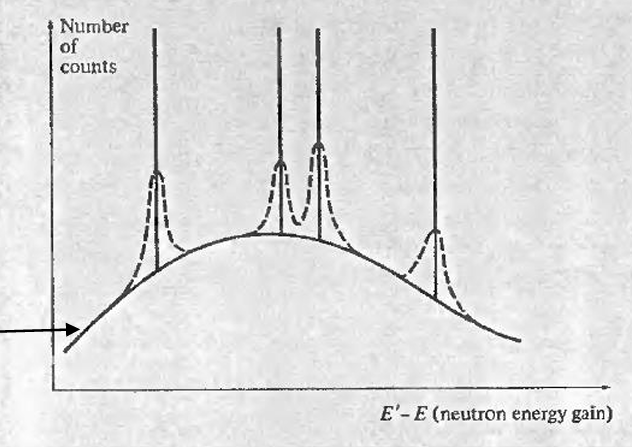
\includegraphics[width=0.7\linewidth]{images/8-Fononi/2phonscatt.png}
    \caption{Spettro di scattering. Il picco intenso corrisponde allo scattering one-phonon, mentre il background continuo evidenzia i processi multi-phonon.}
    \label{fig:2phonon-scattering}
\end{figure}

\section{Conservazione del momento e del momento cristallino}
Dato l'operatore traslazionale $\hat{T}(x) \ket{r} = \ket{r+x}$ l'operatore momento è definito come:
\[ \hat{p} = -i \hbar \left( \vec{\nabla}\hat{T}(x) \right)_{x = 0}\]
considero $\vec{\nabla} T$ come il limite del rapporto incrementale e ho che 
\[ \begin{split}
    & \hat{p_x} = -i\hbar \lim_{a \to 0} \frac{\hat{T}(a\hat{x})-\mathbb{I}}{a} \\
    &(\hat{p}\psi)(r) = -i\hbar \lim_{a \to 0} \frac{(\hat{T}(a)\psi)(r) - \psi(r)}{a} \\
    & = -i\hbar \lim_{a \to 0} \frac{\psi(r-a)-\psi(r)}{a} \\
    & = -i\hbar\frac{\partial}{\partial r} \psi(r)
\end{split}\]
La forma esplicita dell'operatore traslazionale è
\[ \begin{split}
    &\hat{T}(x) = \lim_{N \to \infty} \left( \hat{T} (x/N)\right)^N \\
    &\frac{x}{N} \ \text{è piccolo} \implies \text{espando} \\
    & = \lim_{N \to \infty} \left[ 1-\frac{x}{N}\vec{\nabla} T \right]^N =\\
    & = \lim_{N \to \infty} \left[ 1-\frac{ix\cdot \hat{p}}{N\hbar} \right]^N \\
    & \hat{T}(x) = \exp\left( -\frac{ix\cdot \hat{p}}{\hbar}\right) = 1 - \frac{ix\cdot \hat{p}}{\hbar} - \frac{(x\cdot \hat{p)^2}}{2\hbar^2} + \frac{i(x\cdot \hat{p})^3}{6\hbar^3}+... \\
    & \psi(r-x) = \hat{T}(x)\psi(r) = \exp\left(-  \frac{ix\cdot \hat{p}}{\hbar}\right)\psi(r) = \\
    & = \left( \sum_{n = 0} \frac{1}{n!} \left(  - \frac{i}{\hbar}x \cdot \hat{p}\right)^n\right) \psi(r) = \\
    & = \left( \sum_{n = 0} \frac{1}{n!} \left( -x \cdot\vec{\nabla}\right)^n\right) \psi(r) = \\
    & = \psi(r) - x \cdot \vec{\nabla}\psi(r) + \frac{1}{2!}(x \cdot \vec{\nabla})^2\psi(r)-...
\end{split}\]
La conservazione del momento viene dal fatto che l'hamiltoniana commuta con l'operatore traslazionale:
\[ \begin{split}
    &\left[ \hat{H}, \hat{T}(x) \right] = 0 \\
    & \left[ \hat{H}, 1-\frac{i x \cdot \hat{p}}{N\hbar} \right] = 0 \\
    & \implies \left[ \hat{H}, \hat{p} \right] = 0 \implies \frac{d}{dt}<\hat{p}> = \frac{i}{\hbar}\left[ \hat{H}, \hat{p} \right] = 0
\end{split}\]
In un cristallo la traslazione è data da $\hat{T}(R)$ dove $R$ è un vettore del Bravias lattice
\[ T(R) = e^{ikR} = e^{i(k+K)R}\]
dato che ho $e^{i(k+K)R}$, mi indica che ho un set di vettori siccome $K \in \text{RL}$ quindi p non sarà più ben definito perché ho un insieme di diversi $K$ che mi daranno la stessa traslazione. Quindi è per questo che la conservazione del momento di un cristallo è soddisfatta più o meno un vettore $K$ del reticolo reciproco.


\section{Quantum Harmonic Crystal}
In questo paragrafo calcoliamo il calore specifico a volume costante, \(C_V\), per un solido descritto come un cristallo armonico quantistico. Iniziamo definendo le grandezze macroscopiche fondamentali.
\subsection*{Definizioni Preliminari}
L'energia totale del sistema, dovuta alle vibrazioni quantizzate (fononi), si esprime come:
\begin{equation}
    E_{\text{tot}} = \sum_{n,s} \left(n_s(\mathbf{k}) + \frac{1}{2}\right) \hbar \omega_s(\mathbf{k}),
\end{equation}
dove:
\begin{itemize}
    \item \(n_s(\mathbf{k})\) è il numero di occupazione del fonone nel ramo \(s\) e con vettore d'onda \(\mathbf{k}\);
    \item La presenza del termine \(\frac{1}{2}\) rappresenta l'energia di punto zero, tipica del comportamento quantistico.
\end{itemize}
La distribuzione di Bose-Einstein, che regola la popolazione dei fononi, è data da:
\begin{equation}
    n_s(\mathbf{k}) = \frac{1}{e^{\beta \hbar \omega_s(\mathbf{k})} - 1},
\end{equation}
con \(\beta = \frac{1}{k_B T}\).
L'energia media per unità di volume è:
\begin{equation}
    u(T) = \frac{E_{\text{tot}}}{V},
\end{equation}
e il calore specifico a volume costante è definito come:
\begin{equation}
    C_V = \left(\frac{\partial u(T)}{\partial T}\right)_V.
\end{equation}
Si noti che, in questo contesto, il potenziale chimico \(\mu = 0\) poiché il numero di fononi non è conservato.\\
Riassumendo, possiamo scrivere:
\begin{equation}
    C_V = \frac{1}{V}\sum_{n,s} \frac{\partial}{\partial T} \left[ \hbar \omega_s(\mathbf{k}) \left( \frac{1}{e^{\beta \hbar \omega_s(\mathbf{k})} - 1} + \frac{1}{2} \right) \right].
\end{equation}
\subsection*{Caso Temperature Alte (\(\beta \ll 1\))}
Nel regime delle alte temperature, possiamo espandere la distribuzione di Bose-Einstein per \(x = \beta \hbar \omega\) intorno a \(x=0\). Consideriamo l'espansione:
\begin{equation}
    \frac{1}{e^x - 1} \approx \frac{1}{x + \frac{x^2}{2} + \frac{x^3}{6} + \cdots} \approx \frac{1}{x}\left(1 - \frac{x}{2} + \frac{x^2}{12} + \cdots\right).
\end{equation}
Sostituendo l'espansione nella definizione di \(C_V\) ed esplicitando il termine dell'energia, abbiamo:
\begin{equation}
\begin{split}
    C_V &\approx \frac{1}{V}\sum_{n,s} \frac{\partial}{\partial T} \left[ \hbar \omega_s \left(\frac{k_B T}{\hbar \omega_s} - \frac{1}{2} + \frac{\hbar \omega_s}{k_B T} \cdot \frac{1}{12} \right) \right] \\
    &\approx \frac{1}{V}\sum_{n,s} \left( k_B - \frac{(\hbar \omega_s)^2}{12 k_B} \frac{1}{T^2}\right).
\end{split}
\end{equation}
Dato che, a temperature elevate, ci aspettiamo che il contributo energetico totale sia dominato dal termine costante (secondo il teorema di equipartizione), la somma porta al risultato:
\begin{equation}
    C_V \approx 3R - \frac{1}{V}\sum_{n,s} \frac{(\hbar \omega_s)^2}{12 k_B}\frac{1}{T^2},
\end{equation}
dove \(3R\) rappresenta il contributo classico (in unità di moli, \(R\) è la costante dei gas) e il termine correttivo decresce con \(1/T^2\).

\subsection*{Caso Temperature Basse (\(\beta \gg 1\))}
Nel limite delle basse temperature, i modi vibratori con \(\hbar \omega_s \gg k_B T\) non contribuiscono significativamente all'energia. Inoltre, per basse energie, la relazione di dispersione assume la forma lineare:
\begin{equation}
    \omega_s(\mathbf{k}) \approx c_s\, k,
\end{equation}
con \(c_s\) che rappresenta la velocità del suono nel materiale, e quindi:
\begin{equation}
    x = \beta \hbar c_s k.
\end{equation}
Nel passaggio dal discreto al continuo, la sommatoria si sostituisce con:
\begin{equation}
    \frac{1}{V}\sum_{\mathbf{k}} \to \int \frac{\d\mathbf{k}}{(2\pi)^3}.
\end{equation}
L'energia per unità di volume diventa:
\begin{equation}
\begin{split}
    u(T) &\propto \sum_s \int \frac{\d\mathbf{k}}{(2\pi)^3}\, \hbar \omega_s(\mathbf{k}) \, \frac{1}{e^{\beta \hbar \omega_s(\mathbf{k})} - 1} \\
         &= \sum_s \frac{1}{(2\pi)^3} \cdot 4\pi \int_0^{\infty} \d{k}\, k^2\, \frac{\hbar c_s k}{e^{\beta \hbar c_s k} - 1}.
\end{split}
\end{equation}
Svolgendo il cambio di variabile \(x = \beta \hbar c_s k\), si ottiene:
\begin{equation}
\begin{split}
    u(T) &\propto \sum_s \frac{1}{(2\pi)^3} \cdot 4\pi \int_0^{\infty} \frac{\d{x}}{\beta \hbar c_s}\, \left(\frac{x}{\beta \hbar c_s}\right)^2 \, \frac{\hbar c_s \, \frac{x}{\beta \hbar c_s}}{e^{x} - 1} \\
         &= \sum_s \frac{1}{2\pi^2} \frac{1}{(\beta \hbar c_s)^3} \int_0^{\infty} \frac{x^3}{e^x - 1}\, \d{x}.
\end{split}
\end{equation}
Utilizzando il risultato noto:
\begin{equation}
    \int_0^{\infty} \frac{x^3}{e^x - 1}\, \d{x} = \frac{\pi^4}{15},
\end{equation}
l'energia assume la forma:
\begin{equation}
    u(T) \propto \sum_s \frac{k_B^4}{(\hbar c_s)^3} T^4 \cdot \frac{\pi^4}{15}.
\end{equation}
Il calore specifico a volume costante si ottiene derivando \(u(T)\) rispetto a \(T\):
\begin{equation}
\begin{split}
    C_V &= \frac{\partial u(T)}{\partial T} \propto \sum_s \frac{k_B^4}{(\hbar c_s)^3} \cdot \frac{\pi^4}{15} \cdot 4T^3 \\
    &\propto \frac{2\pi^2}{5}\frac{k_B^4}{(\hbar c_s)^3} T^3.
\end{split}
\end{equation}
Quindi, nel limite delle basse temperature:
\begin{equation}
    C_V \propto T^3,
\end{equation}
in accordo con l'osservazione sperimentale.
\bigskip
\noindent Riassumendo, il comportamento del calore specifico è:
\begin{itemize}
    \item \textbf{A temperature elevate: \(C_V\) tende a un valore costante (con piccole correzioni che decadono come \(1/T^2\)).}
    \item \textbf{A temperature basse: \(C_V \propto T^3\).}
\end{itemize}
